% !Mode:: "TeX:DE:UTF-8:Main"
\documentclass[landscape]{article}
\usepackage{tikzducks,graphicx}
\usepackage[margin=1cm]{geometry}

\newcommand{\towelpath}{%
	(1.1676,0.3641) .. controls (1.1676,0.3641) and (1.3763,0.4825) .. (1.4605,0.4542) .. controls (1.5447,0.4259) and (1.4874,0.2742) .. (1.5769,0.2627) .. controls (1.6664,0.2513) and (1.7126,0.4470) .. (1.8022,0.4655) .. controls (1.8918,0.4839) and (1.9360,0.3787) .. (2.0087,0.4054) .. controls (2.0814,0.4321) and (2.0834,0.4936) .. (2.1476,0.5744) .. controls (2.1292,0.6964) and (1.9783,1.1341) .. (1.8735,1.2390) .. controls (1.6974,1.2913) and (1.2567,1.2394) .. (1.2089,1.1676) .. controls (1.1418,1.0668) and (1.1676,0.3641) .. (1.1676,0.3641) -- cycle;
}

\definecolor{itgreen}{RGB}{0,98,33} 
\definecolor{itgreen}{RGB}{0,140,69}
\definecolor{itred}{RGB}{223,0,36}
\definecolor{itred}{RGB}{205,33,42}
\definecolor{itwhite}{RGB}{244,245,240}
\pagestyle{empty}
\begin{document}
%\tikz[overlay]\node[anchor=north west]{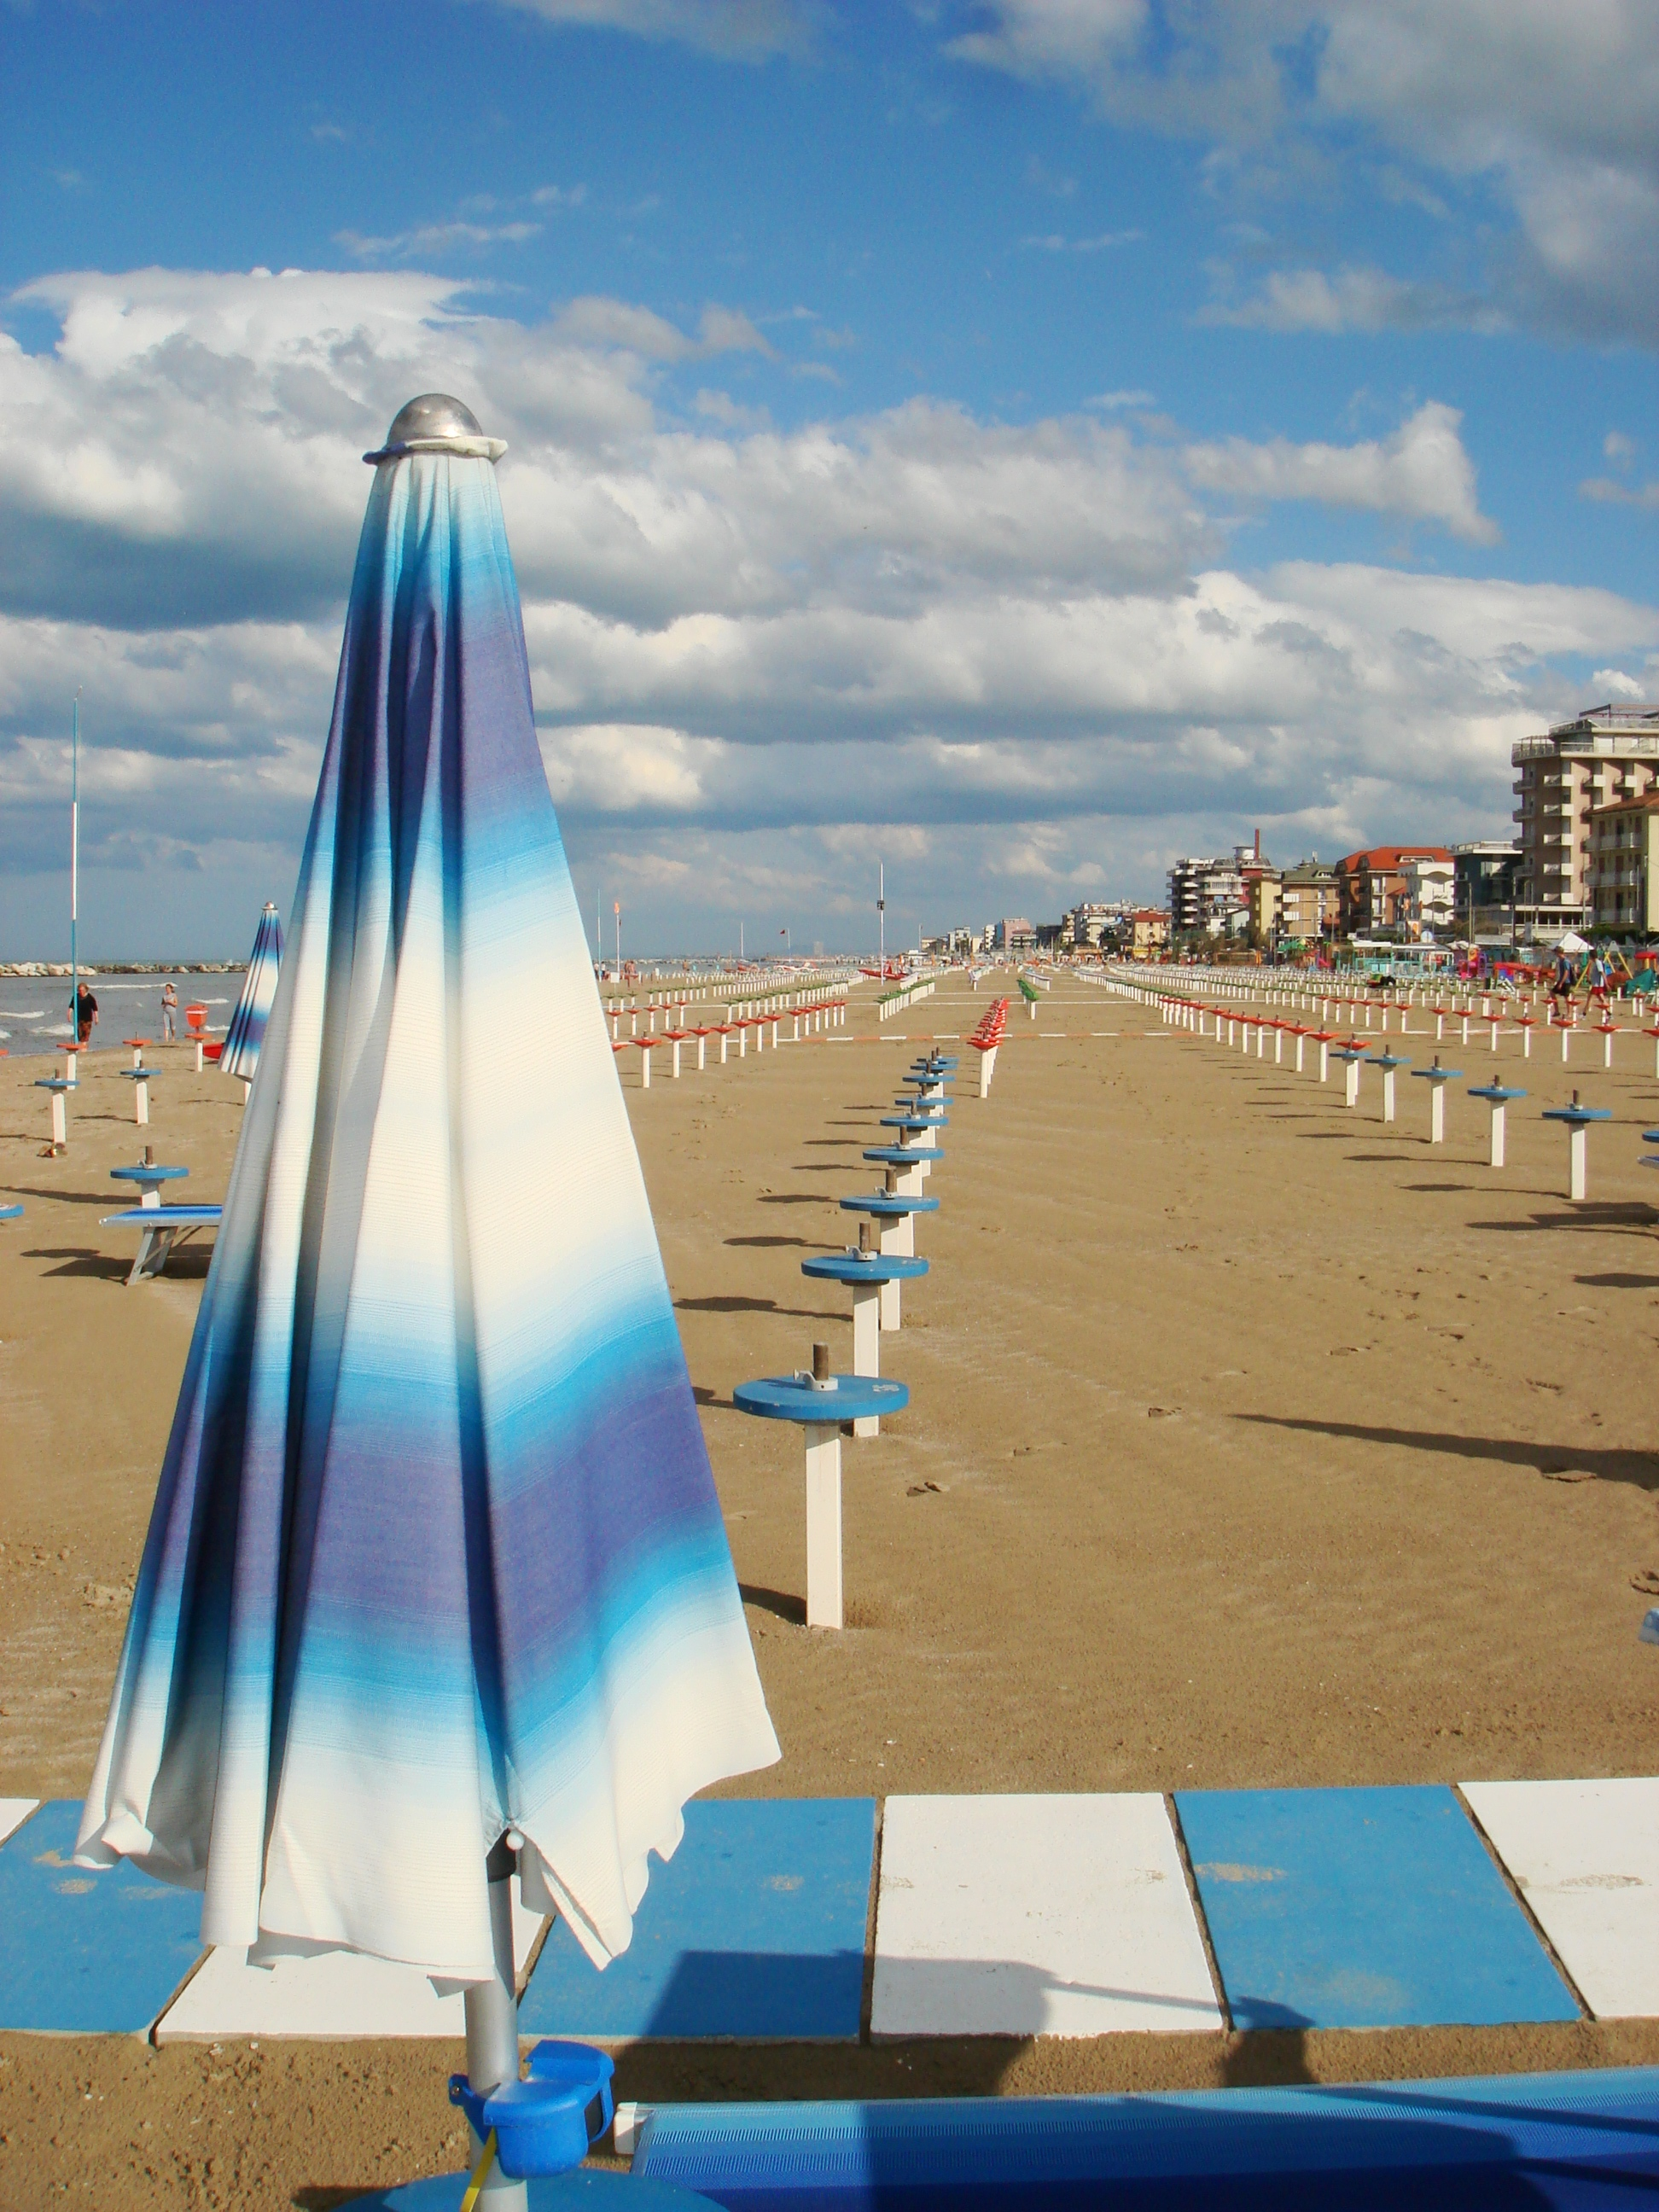
\includegraphics[width=\textwidth]{italy1}};
%\newpage
%
%\tikz[overlay]\node[anchor=north west]{\includegraphics[width=\textwidth]{italy2}};
%\newpage
%beach is https://commons.wikimedia.org/wiki/File:Vespro_-_Mondello_-_33.jpg
\noindent
\begin{tikzpicture}
\node[anchor=south west,inner sep=0pt] (im) {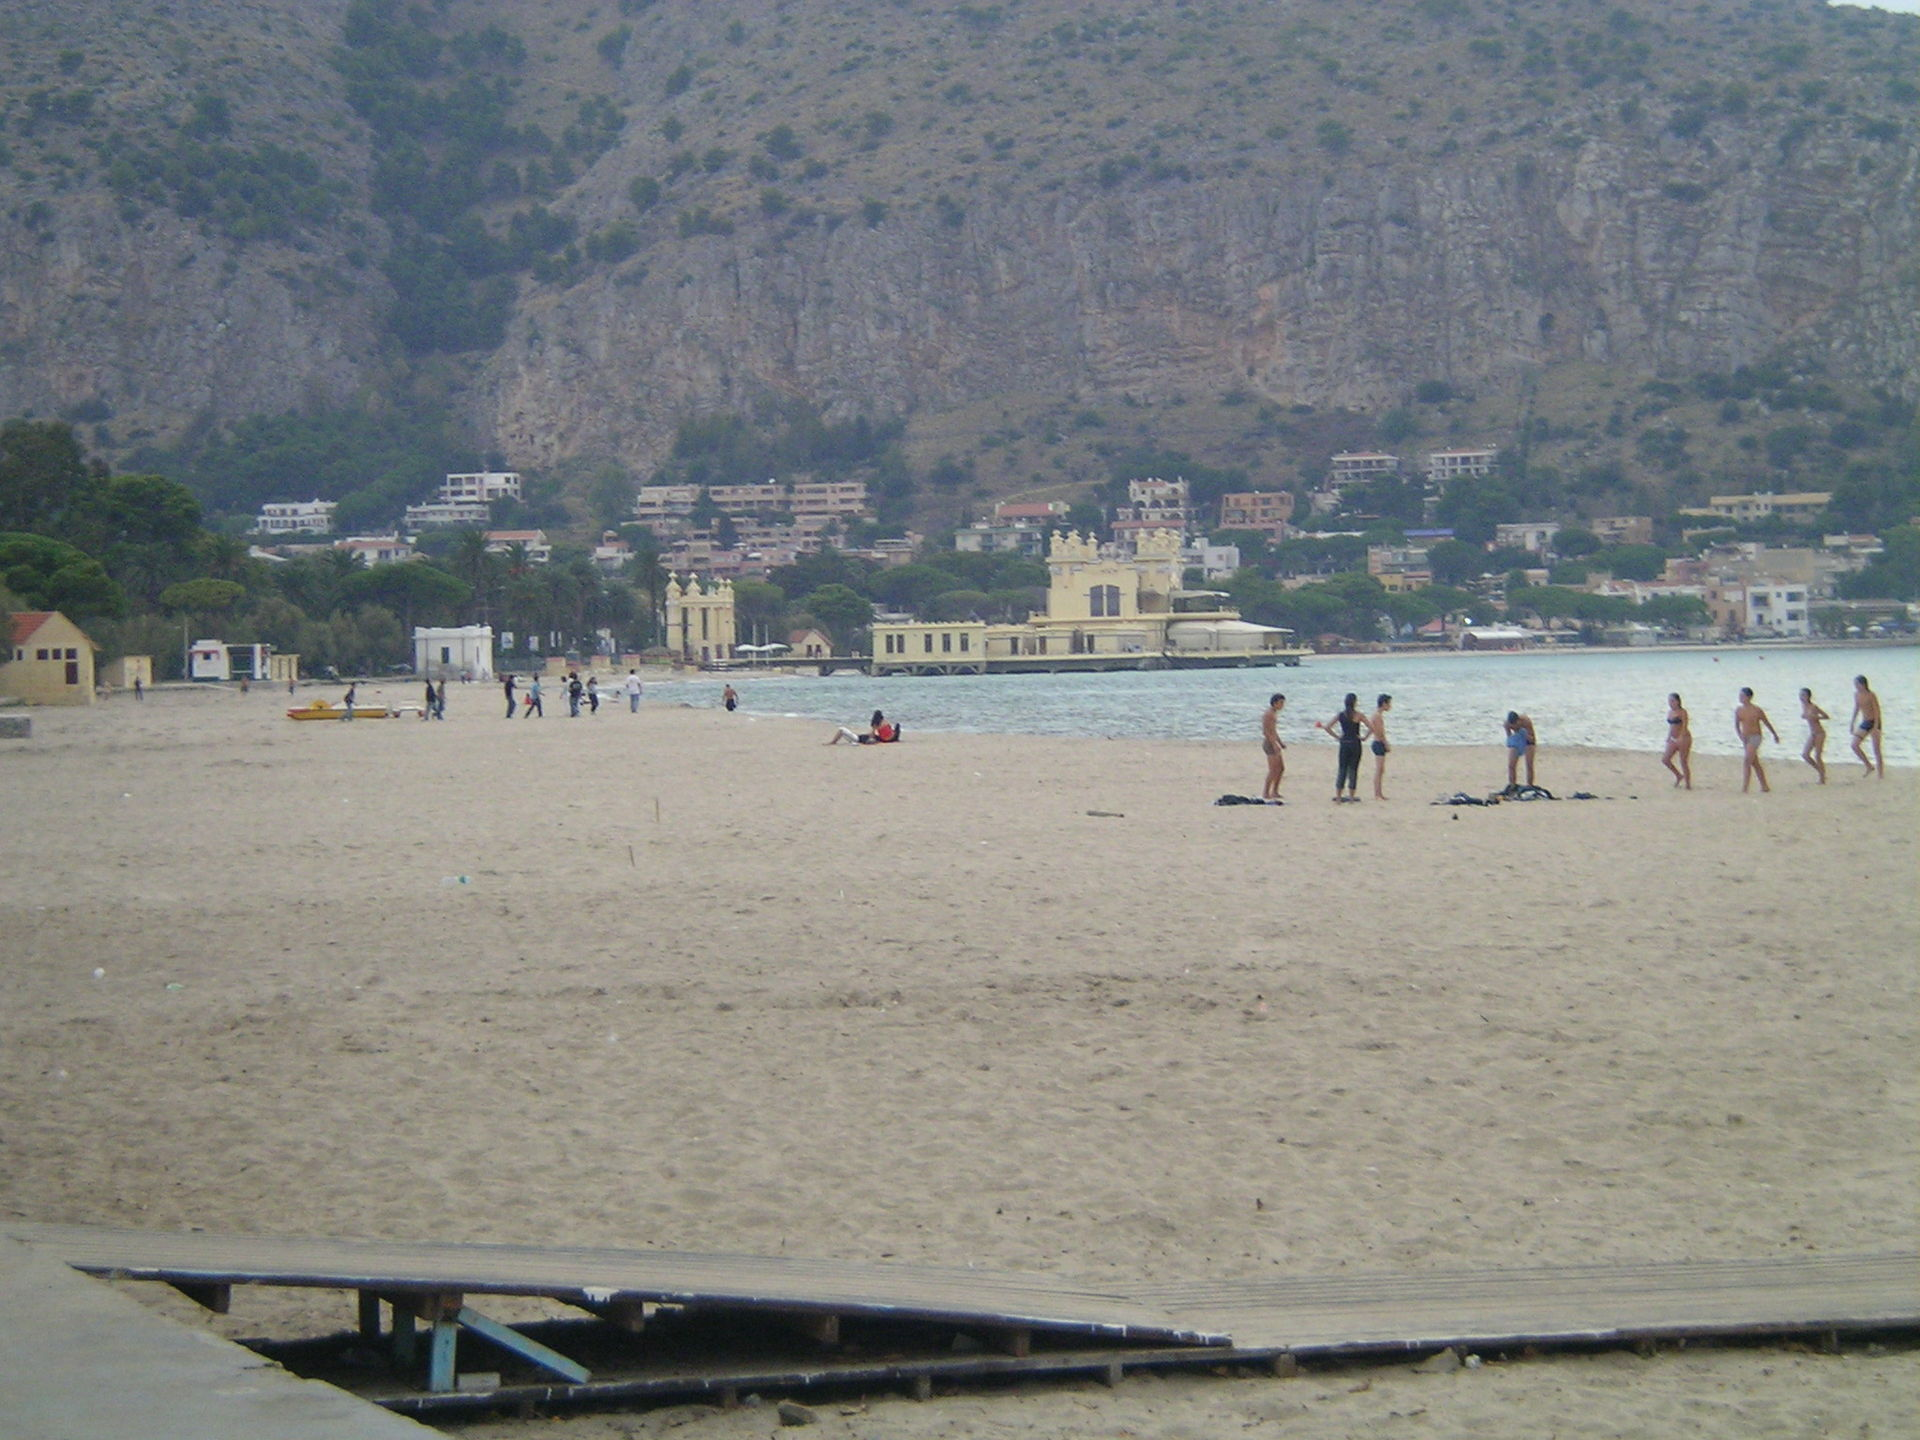
\includegraphics[width=\textwidth,height=\textheight,keepaspectratio]{italy5}};
\path[use as bounding box] (im.south west) rectangle (im.north east);
% duck %%%%%%%%%%%%%%%%%%%%%%%%%%%%%%%%%%%%%%%%%%%%%%%%%%%%%%%%%%%%%%
\begin{scope}[xshift=14cm,yshift=5.5cm]
\begin{scope}[scale=1.05]	
 \duck[%
		cap=itgreen,
		sunglasses,
        book={\scalebox{0.30}{\sffamily\bfseries \begin{tabular}{c}Mondo\\ piccolo\end{tabular}}}
	  ]
% towel %%%%%%%%%%%%%%%%%%%%%%%%%%%%%%%%%%%%%%%%%%%%%%%%%%%%%%%%%%%%%%
	\begin{scope}[scale=0.8,xshift=3mm]
		\fill[cyan!20!white] \towelpath;
		\begin{scope}
			\clip \towelpath;
			\foreach \shifta in {0,0.12,...,2.4}{%
				\fill[white,rotate around={0:(1.2,0.9)}]
				($(0.1,-0.3)+(\shifta,0)$) rectangle ($(0.1,-0.3)+(\shifta,0)+(0.06,2.7)$);
			}
		\end{scope}
	\end{scope}
\end{scope}	
\end{scope}
	
\begin{scope}[xshift=8cm,yshift=7cm]
\begin{scope}[scale=0.8,xscale=-1]
% duck %%%%%%%%%%%%%%%%%%%%%%%%%%%%%%%%%%%%%%%%%%%%%%%%%%%%%%%%%%%%%%
	\duck[%
		strawhat=itred,
        ribbon=itwhite,
		sunglasses,
       book={\scalebox{0.36}{\sffamily\bfseries \begin{tabular}{c}Il\\ gatto-\\pardo \end{tabular}}},
       bookcolor=brown!60!black
	   ]
% towel %%%%%%%%%%%%%%%%%%%%%%%%%%%%%%%%%%%%%%%%%%%%%%%%%%%%%%%%%%%%%%
	\begin{scope}[scale=0.8,xshift=3mm]
		\fill[itgreen!60!white] \towelpath;
		\begin{scope}
			\clip \towelpath;
			\foreach \shifta in {0,0.12,...,2.4}{%
				\fill[white,rotate around={0:(1.2,0.9)}]
				($(0.1,-0.3)+(\shifta,0)$) rectangle ($(0.1,-0.3)+(\shifta,0)+(0.06,2.7)$);
			}
		\end{scope}
	\end{scope}
% book %%%%%%%%%%%%%%%%%%%%%%%%%%%%%%%%%%%%%%%%%%%%%%%%%%%%%%%%%%%%%%%
\end{scope}	
\end{scope}

\begin{scope}[xshift=4cm,yshift=6cm]%ok
\begin{scope}[scale=1.1,xscale=-1]
% duck %%%%%%%%%%%%%%%%%%%%%%%%%%%%%%%%%%%%%%%%%%%%%%%%%%%%%%%%%%%%%%
	\duck[%
		strawhat=itgreen,
        ribbon=itwhite,
		sunglasses,
        icecream=brown,
        flavoura=green!50!brown,
        flavourb=white,
        flavourc=red]
	   % towel %%%%%%%%%%%%%%%%%%%%%%%%%%%%%%%%%%%%%%%%%%%%%%%%%%%%%%%%%%%%%%
	\begin{scope}[scale=0.8,xshift=3mm]
		\fill[itred] \towelpath;
		\begin{scope}
			\clip \towelpath;
			\foreach \shifta in {0,0.12,...,2.4}{%
				\fill[white,rotate around={0:(1.2,0.9)}]
				($(0.1,-0.3)+(\shifta,0)$) rectangle ($(0.1,-0.3)+(\shifta,0)+(0.06,2.7)$);
			}
		\end{scope}
	\end{scope}
\end{scope}
\end{scope}


\begin{scope}[xshift=21cm,yshift=5cm]%ok
\begin{scope}[scale=1]
% duck %%%%%%%%%%%%%%%%%%%%%%%%%%%%%%%%%%%%%%%%%%%%%%%%%%%%%%%%%%%%%%
	\duck[%
		strawhat=itwhite,
        ribbon=itred,
		sunglasses,
       wine=red!50!black]
	
% towel %%%%%%%%%%%%%%%%%%%%%%%%%%%%%%%%%%%%%%%%%%%%%%%%%%%%%%%%%%%%%%
	\begin{scope}[scale=0.8,xshift=3mm]
		\fill[cyan!20!white] \towelpath;
		\begin{scope}
			\clip \towelpath;
			\foreach \shifta in {0,0.12,...,2.4}{%
				\fill[white,rotate around={0:(1.2,0.9)}]
				($(0.1,-0.3)+(\shifta,0)$) rectangle ($(0.1,-0.3)+(\shifta,0)+(0.06,2.7)$);
			}
		\end{scope}
	\end{scope}
% book %%%%%%%%%%%%%%%%%%%%%%%%%%%%%%%%%%%%%%%%%%%%%%%%%%%%%%%%%%%%%%%
	
\end{scope}	
\end{scope}
\begin{scope}[xshift=17cm,yshift=1.5cm]%ok
\begin{scope}[scale=1.6]
% duck %%%%%%%%%%%%%%%%%%%%%%%%%%%%%%%%%%%%%%%%%%%%%%%%%%%%%%%%%%%%%%
	\duck[%
		cap=itred,
        ribbon=itwhite,
		sunglasses,
book={\scalebox{0.36}{\sffamily\bfseries \begin{tabular}{c}\\Il\\nome\\ della\\ rosa\end{tabular}}}]
	
% towel %%%%%%%%%%%%%%%%%%%%%%%%%%%%%%%%%%%%%%%%%%%%%%%%%%%%%%%%%%%%%%
	\begin{scope}[scale=0.8,xshift=3mm]
		\fill[itgreen] \towelpath;
		\begin{scope}
			\clip \towelpath;
			\foreach \shifta in {0,0.12,...,2.4}{%
				\fill[white,rotate around={0:(1.2,0.9)}]
				($(0.1,-0.3)+(\shifta,0)$) rectangle ($(0.1,-0.3)+(\shifta,0)+(0.06,2.7)$);
			}
		\end{scope}
	\end{scope}
\end{scope}
\end{scope}
\begin{scope}[xshift=11cm,yshift=2cm]%ok
\begin{scope}[scale=1.6,xscale=-1]
% duck %%%%%%%%%%%%%%%%%%%%%%%%%%%%%%%%%%%%%%%%%%%%%%%%%%%%%%%%%%%%%%
	\duck[%
		cap=itwhite,
        ribbon=itwhite,
		sunglasses,
       milkshake]
	
% towel %%%%%%%%%%%%%%%%%%%%%%%%%%%%%%%%%%%%%%%%%%%%%%%%%%%%%%%%%%%%%%
	\begin{scope}[scale=0.8,xshift=3mm]
		\fill[itgreen] \towelpath;
		\begin{scope}
			\clip \towelpath;
			\foreach \shifta in {0,0.12,...,2.4}{%
				\fill[white,rotate around={0:(1.2,0.9)}]
				($(0.1,-0.3)+(\shifta,0)$) rectangle ($(0.1,-0.3)+(\shifta,0)+(0.06,2.7)$);
			}
		\end{scope}
	\end{scope}
\end{scope}
\end{scope}
\end{tikzpicture}
\end{document}